\documentclass{article}\usepackage[]{graphicx}\usepackage[]{color}
%% maxwidth is the original width if it is less than linewidth
%% otherwise use linewidth (to make sure the graphics do not exceed the margin)
\makeatletter
\def\maxwidth{ %
  \ifdim\Gin@nat@width>\linewidth
    \linewidth
  \else
    \Gin@nat@width
  \fi
}
\makeatother

\definecolor{fgcolor}{rgb}{0.345, 0.345, 0.345}
\newcommand{\hlnum}[1]{\textcolor[rgb]{0.686,0.059,0.569}{#1}}%
\newcommand{\hlstr}[1]{\textcolor[rgb]{0.192,0.494,0.8}{#1}}%
\newcommand{\hlcom}[1]{\textcolor[rgb]{0.678,0.584,0.686}{\textit{#1}}}%
\newcommand{\hlopt}[1]{\textcolor[rgb]{0,0,0}{#1}}%
\newcommand{\hlstd}[1]{\textcolor[rgb]{0.345,0.345,0.345}{#1}}%
\newcommand{\hlkwa}[1]{\textcolor[rgb]{0.161,0.373,0.58}{\textbf{#1}}}%
\newcommand{\hlkwb}[1]{\textcolor[rgb]{0.69,0.353,0.396}{#1}}%
\newcommand{\hlkwc}[1]{\textcolor[rgb]{0.333,0.667,0.333}{#1}}%
\newcommand{\hlkwd}[1]{\textcolor[rgb]{0.737,0.353,0.396}{\textbf{#1}}}%
\let\hlipl\hlkwb

\usepackage{framed}
\makeatletter
\newenvironment{kframe}{%
 \def\at@end@of@kframe{}%
 \ifinner\ifhmode%
  \def\at@end@of@kframe{\end{minipage}}%
  \begin{minipage}{\columnwidth}%
 \fi\fi%
 \def\FrameCommand##1{\hskip\@totalleftmargin \hskip-\fboxsep
 \colorbox{shadecolor}{##1}\hskip-\fboxsep
     % There is no \\@totalrightmargin, so:
     \hskip-\linewidth \hskip-\@totalleftmargin \hskip\columnwidth}%
 \MakeFramed {\advance\hsize-\width
   \@totalleftmargin\z@ \linewidth\hsize
   \@setminipage}}%
 {\par\unskip\endMakeFramed%
 \at@end@of@kframe}
\makeatother

\definecolor{shadecolor}{rgb}{.97, .97, .97}
\definecolor{messagecolor}{rgb}{0, 0, 0}
\definecolor{warningcolor}{rgb}{1, 0, 1}
\definecolor{errorcolor}{rgb}{1, 0, 0}
\newenvironment{knitrout}{}{} % an empty environment to be redefined in TeX

\usepackage{alltt}
\usepackage{Sweave}
\usepackage{tabularx}
\usepackage{geometry}
\geometry{margin=.5in}
\usepackage{enumerate}
\usepackage[demo]{graphicx}
\makeatletter
\setlength{\@fptop}{0pt}
\makeatother
\IfFileExists{upquote.sty}{\usepackage{upquote}}{}
\begin{document}

\section*{Introduction}
Bias correction needed (see figure 1)
\section*{Methods}
formula for bias correction

\section*{Results and Findings}
Fake data actual values: intercept 8,slope=.1
mean over all species: mean spint, mean speff
It is good! see?\\
formula: bvol ~ doy + (doy | sp)
------

Estimates:
            Median MAD_SD
(Intercept) 8.3    1.4   
doy         0.1    0.0   
sigma       4.1    0.1 

TO DO: CALCULTE 95 CI

\subsection{Modeling temporal bias and correction}
formula: log_bvol ~ doy + (doy | name)
------

Estimates:
            Median MAD_SD
(Intercept) 0.3    0.3   
doy         0.0    0.0   
sigma       1.4    0.0

##make this into a table
> coef(truvol)
$name
                          (Intercept)           doy
Acer_pensylvanicum         0.97458062  0.0135474656
Acer_rubrum               -0.87769216  0.0178379549
Acer_saccharum            -0.33066940 -0.0085356410
Alnus_incana               1.91813397  0.0033483077
Aronia_melanocarpa        -1.12912393 -0.0021545908
Betula_alleghaniensis      1.73879663  0.0023795954
Betula_lenta               1.98438474 -0.0021823538
Betula_papyrifera          1.75282749  0.0057429543
Corylus_cornuta            0.16674931  0.0105563237
Fagus_grandifolia         -0.14653414  0.0179099137
Fraxinus_nigra             0.92681574  0.0001589012
Hamamelis_virginiana       0.37882207 -0.0008616836
Ilex_mucronata            -0.86021753  0.0078131211
Lonicera_canadensis       -1.47947450  0.0227057059
Lyonia_ligustrina          0.08967601  0.0058018335
Nyssa_sylvatica            0.29961298  0.0067295703
Populus_grandidentata      2.79094437 -0.0095892349
Prunus_pensylvanica       -0.82793248  0.0098234703
Quercus_alba               0.45222579 -0.0164645539
Quercus_rubra              0.22698585  0.0048372103
Quercus_velutina           0.77476146  0.0002200500
Rhamnus_frangula          -0.10823800  0.0045472003
Rhododendron_prinophyllum -1.12736218  0.0060342932
Spiraea_alba              -0.67236604 -0.0041050694
Vaccinium_myrtilloides    -2.38204936  0.0059859085
Viburnum_cassinoides      -0.40934429  0.0064627936
Viburnum_lantanoides       4.21958712 -0.0011653093




\begin{figure}[h!]
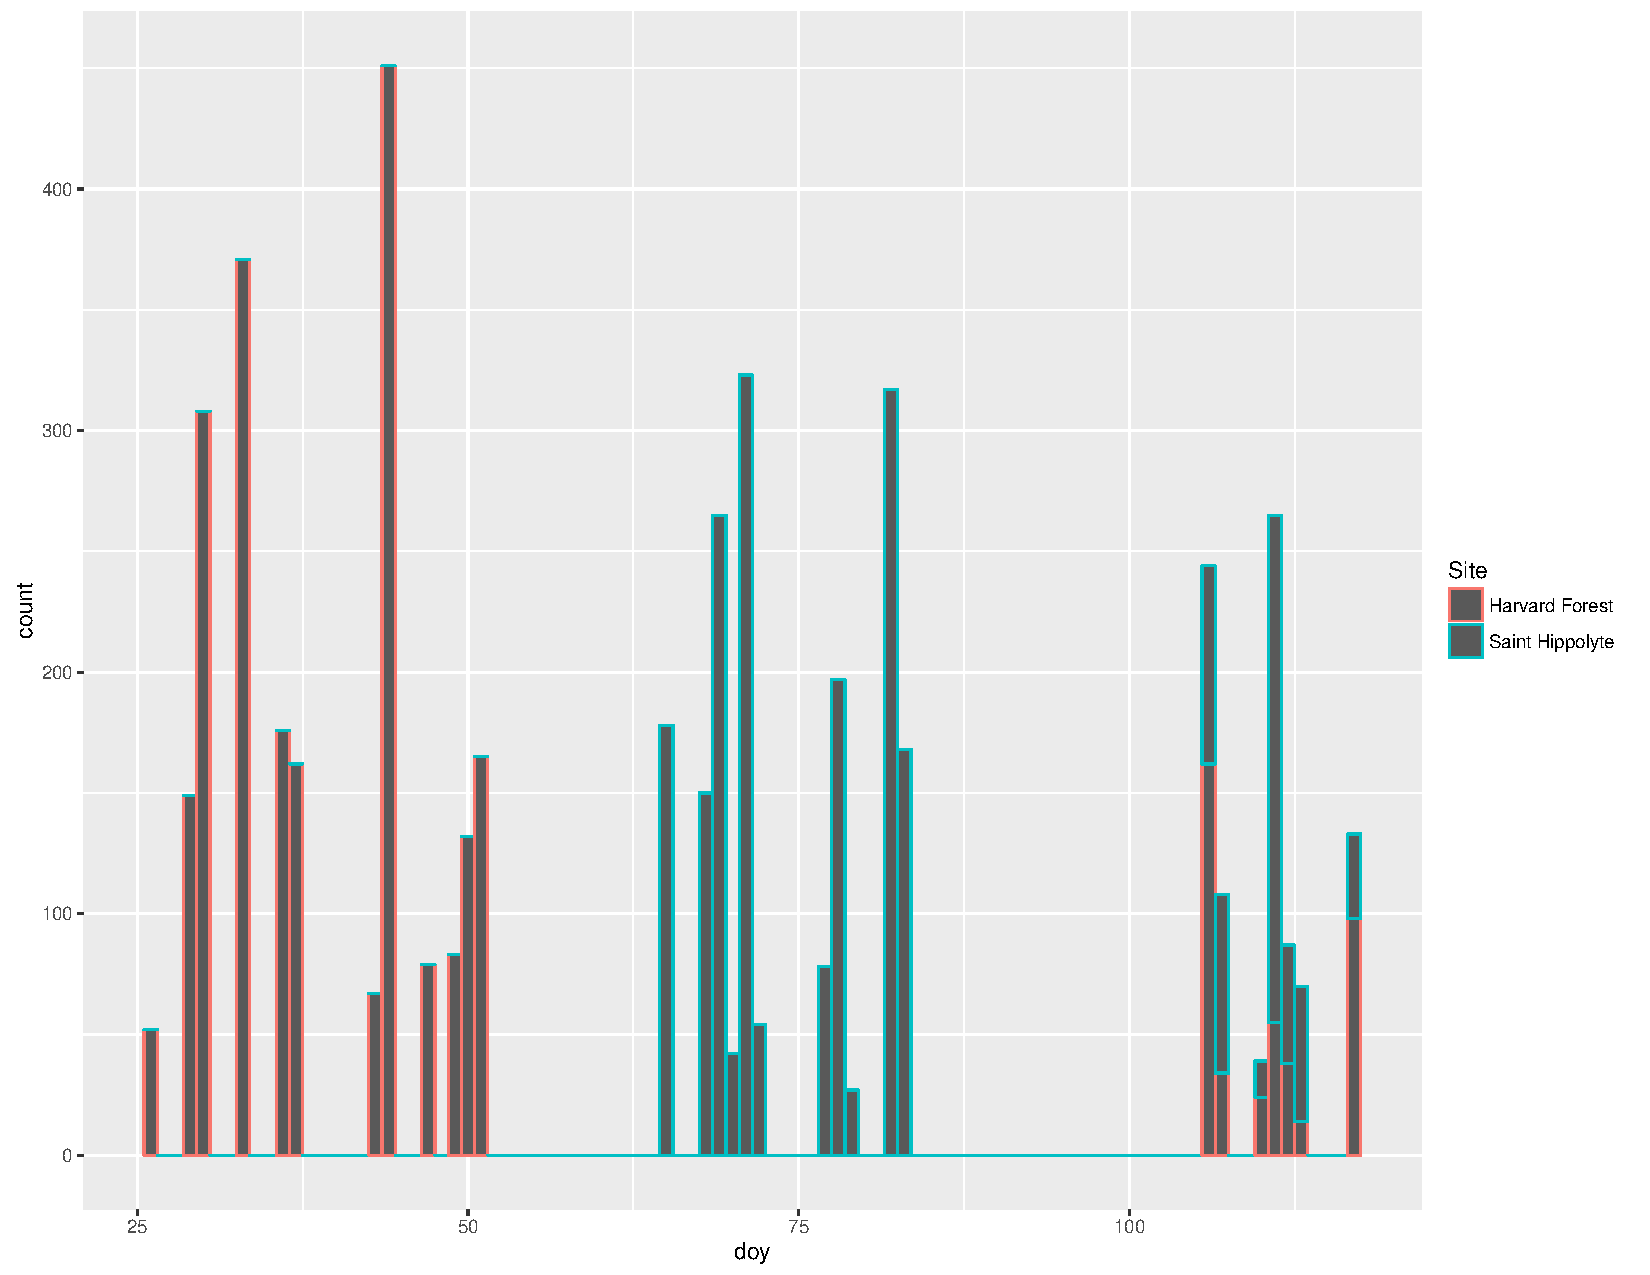
\includegraphics[width=15cm, height=15cm]{temp_bias_fig.pdf}\\
\caption{Measurement days of buds colored by site. Twigs from the different site were measured non-randomly, producing a temporal bias}
\end{figure}

\begin{figure}[h!]
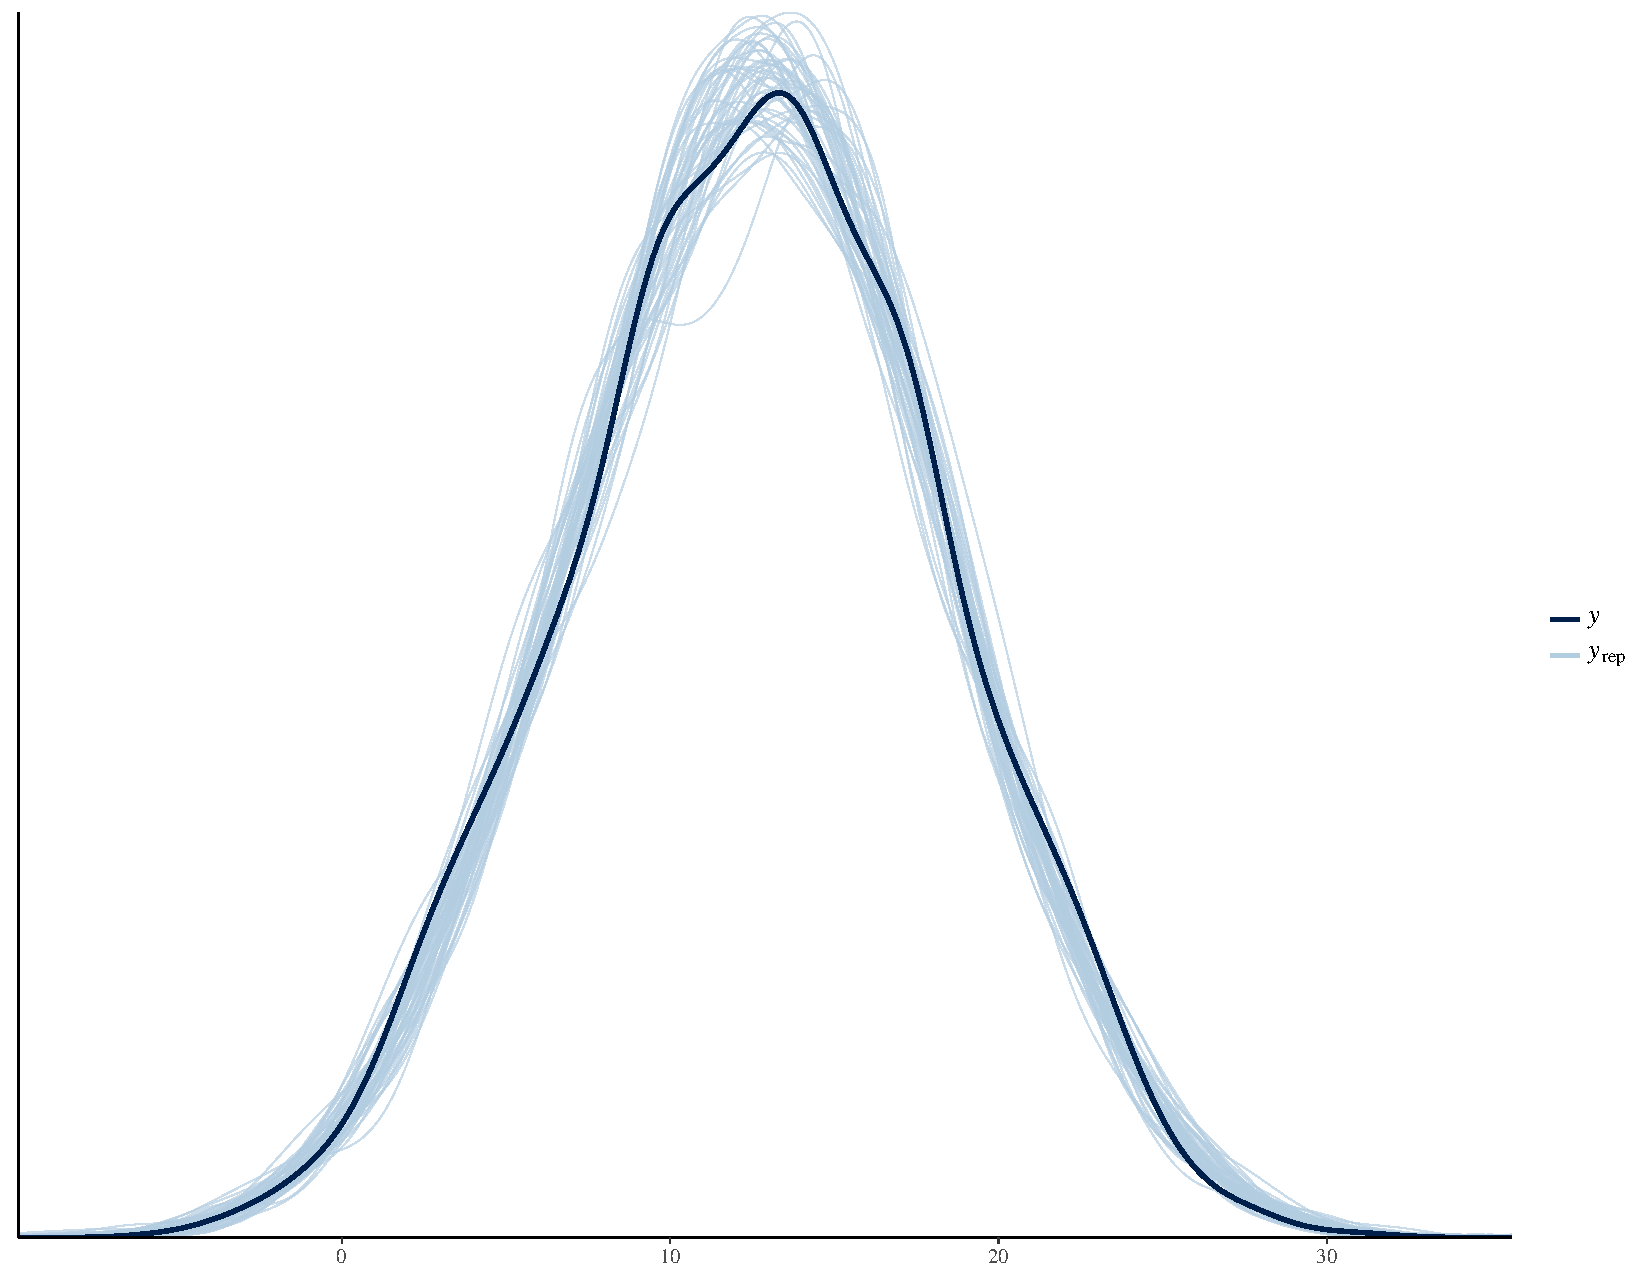
\includegraphics[width=15cm, height=15cm]{fake_data_pp_check_final.pdf}\\
\caption{Posterior predictive checks for model bvol ~ doy + (doy | sp) on fake data}
\end{figure}

\begin{figure}[h!]
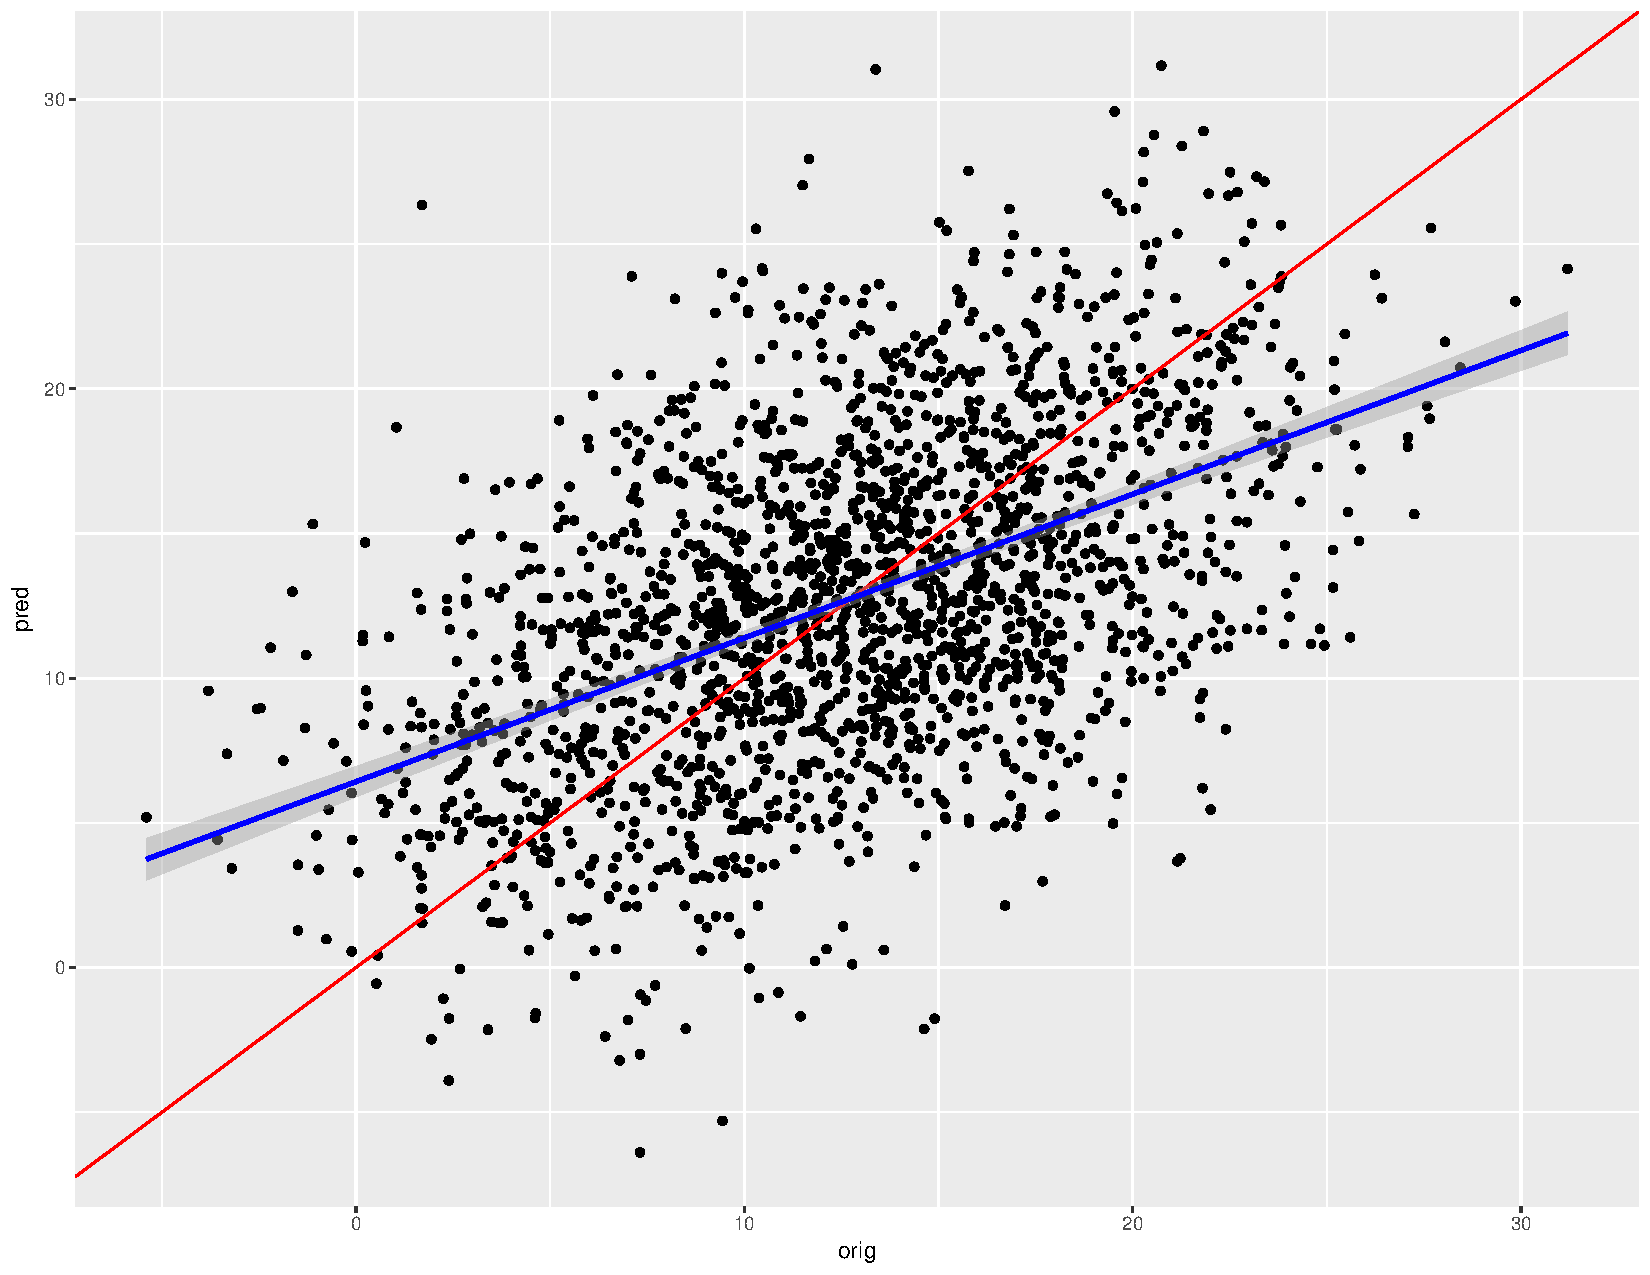
\includegraphics[width=15cm, height=15cm]{fake_predvsorig_final.pdf}\\
\caption{Predicted vs. original values for fake data. The red line represents the 1:1 line which would represent perfect prediction. The blue line is the actual slope, demonstration some deviation}
\end{figure}

\begin{figure}[h!]
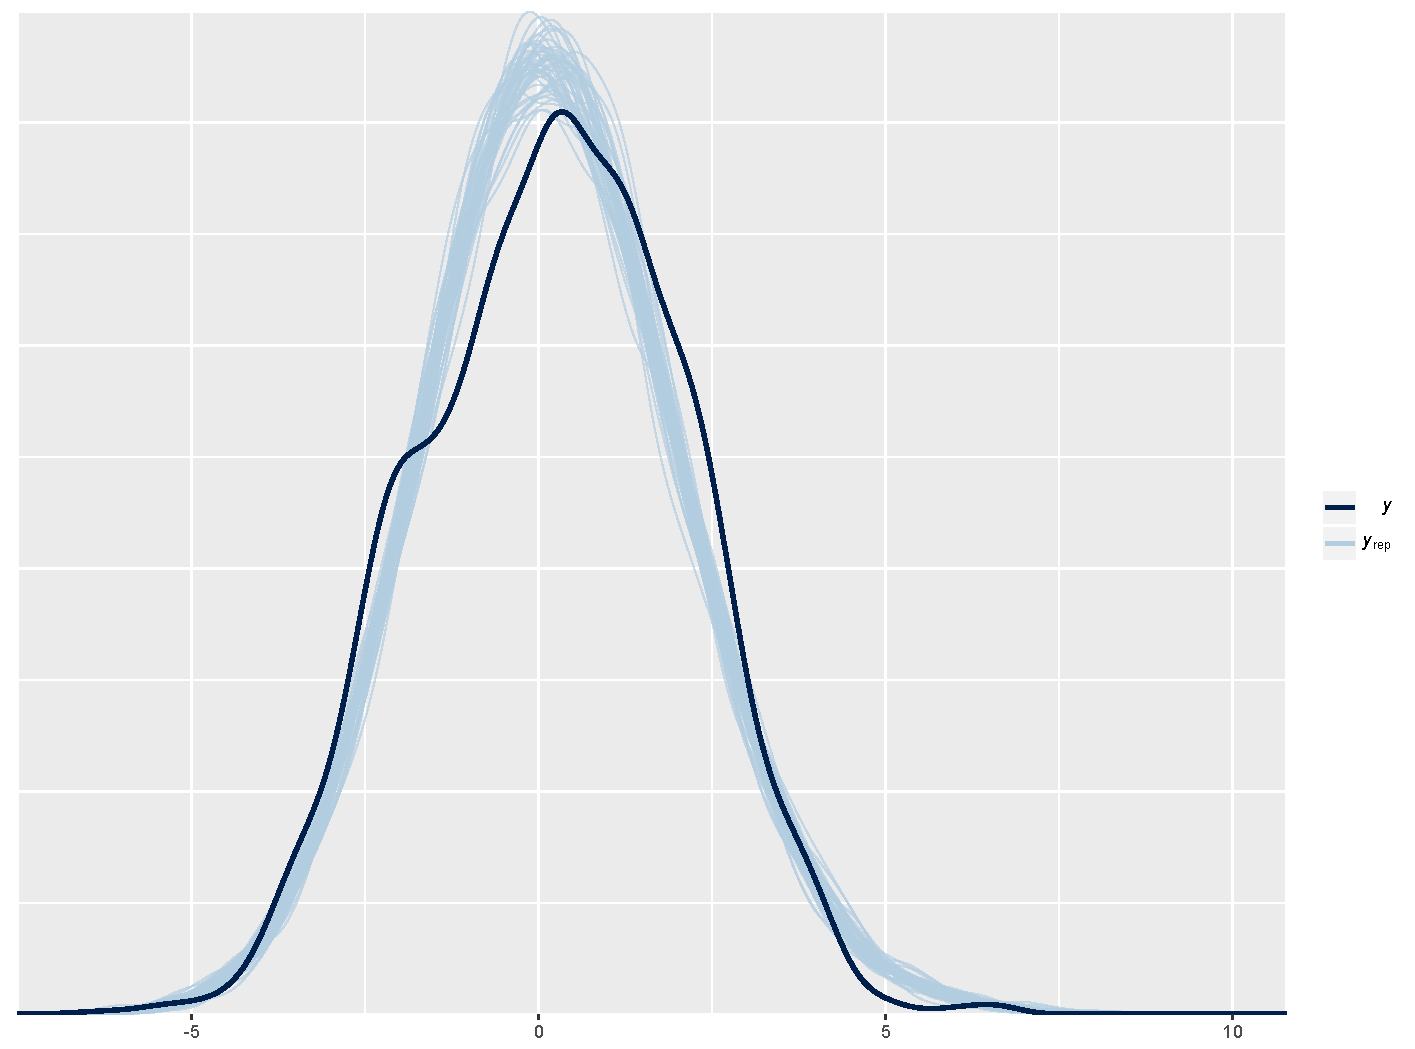
\includegraphics[width=15cm, height=15cm]{pp_check_log_real.pdf}\\
\caption{Posterior predictive checks for model bvol ~ doy + (doy | sp) on real data}
\end{figure}







\end{document}
